\documentclass[12pt,a4paper]{article}
\pagestyle{plain}
\usepackage{fullpage}
\usepackage[english]{babel}
\usepackage{enumerate}

%equations
\usepackage[fleqn]{amsmath}
\numberwithin{equation}{section}

%figures
\usepackage[dvips]{graphicx}
\graphicspath{{./images/}}
\numberwithin{figure}{section}

%excercises
\newcounter{Exercise}
\setcounter{Exercise}{1}
\usepackage[dvipsnames]{xcolor}
\usepackage{framed}
\definecolor{shadecolor}{gray}{0.9}
\usepackage{caption}

%tables
\numberwithin{table}{section}

%specials
\usepackage{textcomp} %special (greek) characters as text
%\usepackage{pstricks} %
%\usepackage{ifthen} %
%\usepackage{calc} %
%\usepackage{isotope}
\usepackage{hyperref}
\usepackage[bottom]{footmisc} %footnote below figure
\usepackage{footnpag}%number footnotes per page


%document details
\author{Koos Kortland \\ translated and adapted by K. Schadenberg}
\date{}
\title{HiSPARC Detector - Detector Station}


\begin{document}
\maketitle

\section{Introduction}
This module is a part of a series describing the HiSPARC detector.

A detector station consists of two or four detectors connected via an electronics box to a computer an a GPS antenna. A detector station gathers a large amount of data. In this text we will discuss how to sort through this data and only save the relevant information.

\section{Station Types}
A single detector station can either have two or four detectors. Below is a short description of the different setups.
\begin{description}
\item [Two plate setup] A two setup has two detectors spaced 10 metres apart, the GPS antenna is placed between the plates. This setup is the simplest configuration able to detect cosmic showers.
\item [Two plate setup - Triangle] Four detectors are placed on a equilateral triangle, three on the corners and one in the centroid. The GPS antenna is placed close to the centroid. The direction of the primary particle can be reconstructed if secondary particles are detected by at least three of the four plates.  If all four plates are struck by particles, the detector can be seen as three smaller triangular shaped detector stations, allowing for an estimation of the error in the angle reconstruction.
\item [Two plate setup - Rhombus] Four detectors are placed on the corners of a rhombus with the GPS antenna placed in the centre. Like in the triangular setup, if at least three detectors register particles coming from a single shower the direction of the primary particle can be determined. The orientation of the setup changes the sensitivity of the detector station to shower direction.
\end{description}

\section{Data Collection}
For the remainder of this text we will only look at the two detector setup.

The scintillator plates in the detectors are constantly struck by muons. Most of them are not created by high energetic cosmic rays but are the result of less energetic processes. The count rate of a single plate in is the order of magnitude of $10^2$. The plates connected to the computer thus create a large amount of data. However we are only interested in particles coming from air showers. We need to filter the data to only register or save this data. To do this we use the simultaneity of arriving muons. Muons created by an air shower will reach the surface of the Earth at roughly the same time. We will therefore only collect data when both plates register a passing particle within a time frame of 1~$\mu$s ($10^{-6}$~s), we call this a \emph{coincidence} (from coinciding, not by chance). 

An electronic circuit, drawn in figure~\ref{fig:station_schematic}, is used to detect the coincidences. It consists of two comparators and an AND-gate. If a plate detects the passing of a particle the voltage coming from the PMT will pass the threshold set to the comparator. Only if both signals coming from the plates surpass the threshold will the AND-gate trigger the storing of the data coming from the PMTs together with the GPS time stamp. What is stored is a possible air shower. 

\begin{figure}\begin{center}
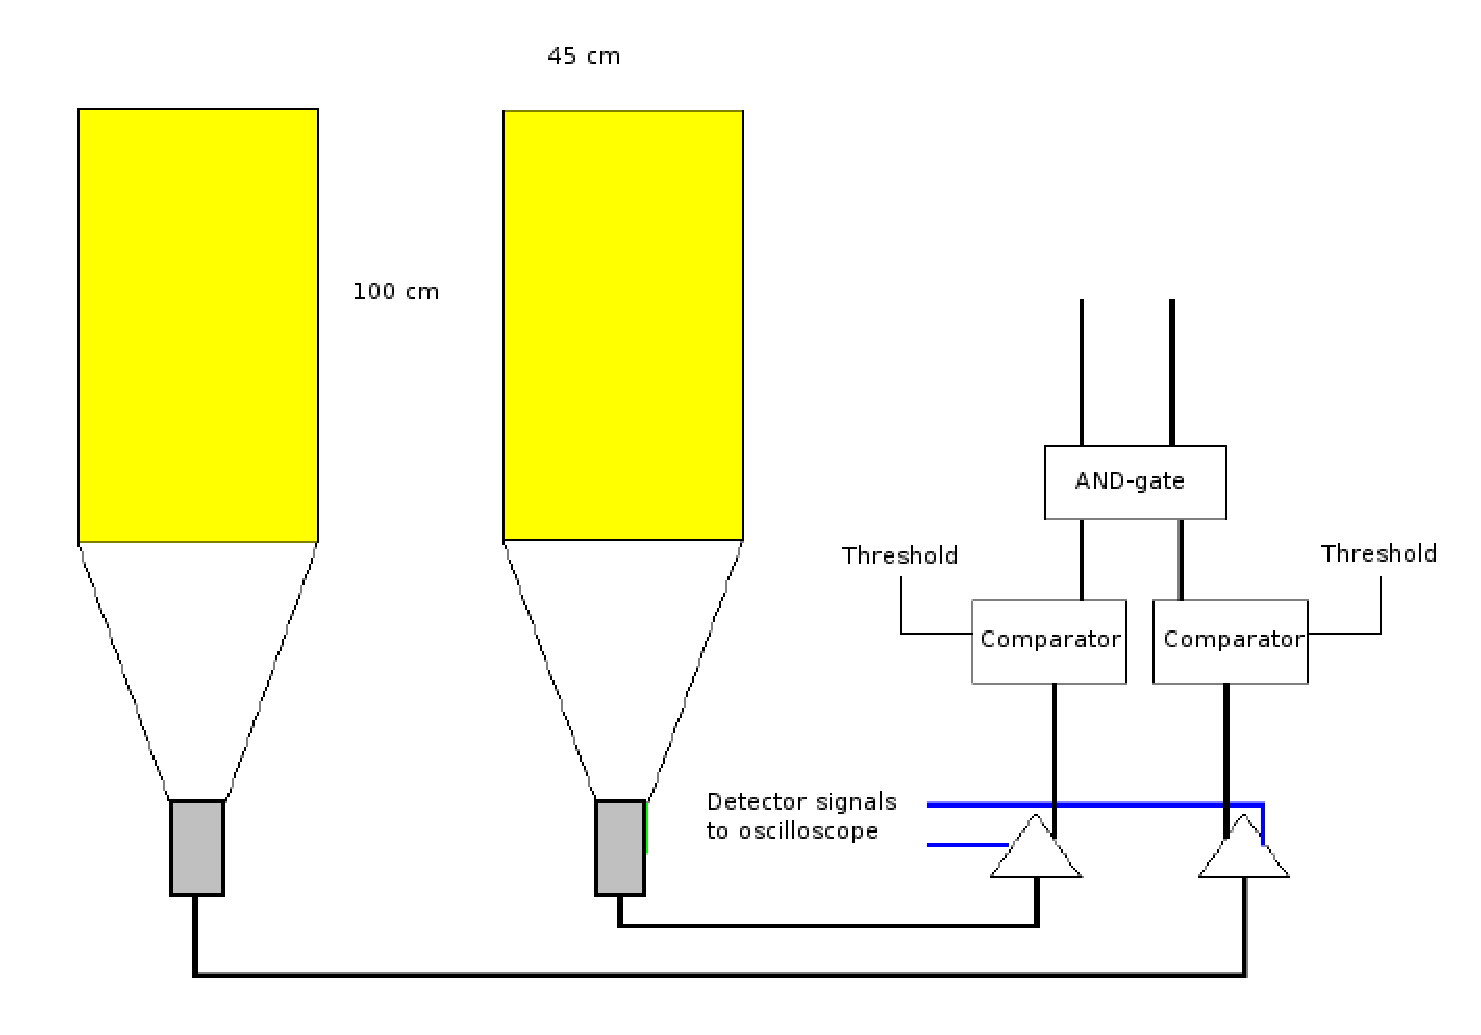
\includegraphics[scale=0.65]{station_schematic.eps}%
\caption{Schematic representation of a two plate HiSPARC detector station and processing electronics. }\label{fig:station_schematic}
\end{center}\end{figure}

Using the logical circuit greatly reduces the amount data to be saved. The time window of 1~$\mu$s is chosen because it is the expected maximum time difference between muons created in the same shower. A simulation of the coincidence-circuit can be found at:
\url{hisparc.nl/en/docent-student/hisparc-detector/}

\section{Real Showers}
The logical circuit described in the previous section selects possible showers. But how can we be certain we really measured an air shower created by a high energetic cosmic particle? Perhaps we measured a mini-shower created by the more frequent low energetic cosmic rays. To see verify whether or not we measured an extensive air shower we need to look at the data from nearby detector stations. If they also measured a possible shower at the exact same time we can be fairly certain it was an extensive air shower.

This is were the importance of the GPS antenna comes into play. HiSPARC uses GPS as a very accurate clock, allowing us the relate events near one detector station to events at a different station. We can set the clocks of our measuring computers with an accuracy of a few dozen of nanoseconds. The GPS antenna also gives us the exact location of the detector station.

Data collected by the computer is sent via an internet to a central storage server at NIKHEF in Amsterdam. Here the data from all individual detector stations is combined to allow for data processing. It is also made available via the HiSPARC website. We can for instance look for coincidence signals from different detector stations within a time window of 1~$\mu$s. An example of such an event is shown in figure~\ref{fig:multiple_coin}.

\begin{figure}\begin{center}
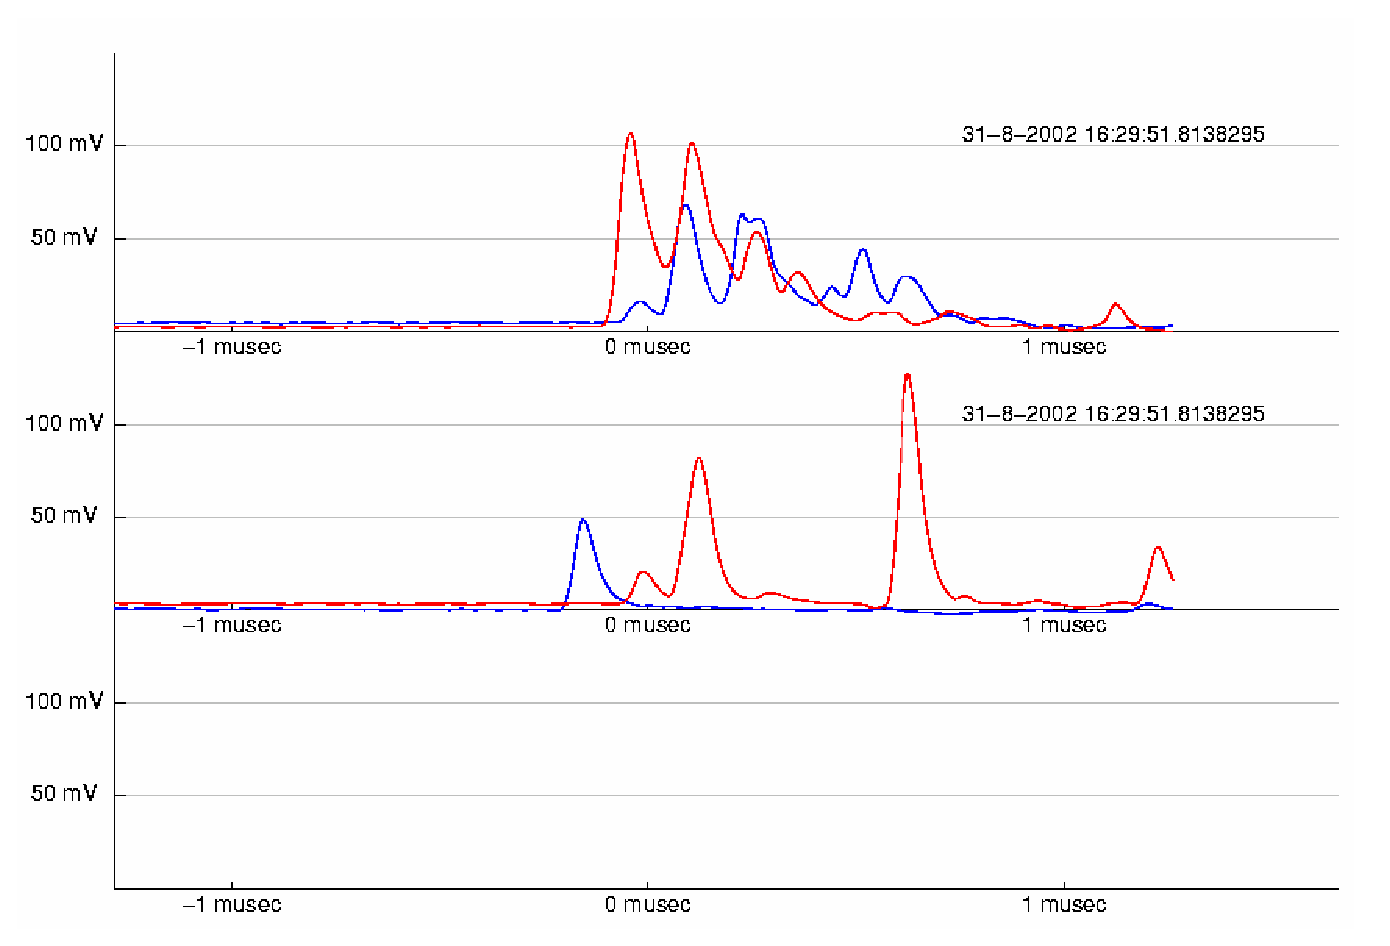
\includegraphics[scale=0.65]{multiple_coin.eps}
\caption{Signals from a multiple coincidence at two detector stations in the Nijmegen cluster. The signals from the oscilloscope are colour red and blue for the different detector plates in both station. The diagram shows the pulse height in mV as a function of the time. Clearly this is an event asking for further investigation. A `normal' event would show a single clear peak in all detector plates.\protect\footnotemark}\label{fig:multiple_coin}
\end{center}\end{figure}

\footnotetext{The Nijmegen cluster is a bit older than the other clusters. HiSPARC started out as the NAHSA project (Nijmegen Area High School Array). This predecessor of HiSPARC used a different version of the electronics boxed currently used. These Nijmegen results show positive peaks whereas the new HiSPARC electronics boxes report negative peaks.}

\section{Coincidental Coincidences}
Our logical circuit might also trigger in the absence of the shower, large or small. Both plates connected to the station might be hit by different and unrelated particles but within the set time window. This is a `false' reading, noise. How often do we measure such a false shower?

\begin{shaded}
\textbf{Exercise \theExercise \stepcounter{Exercise}} : The count rate of random coincidences can be calculated if we know a bit more about the particles triggering our detectors. Suppose the count rate of detector A and B are $f_A$ and $f_B$ respectively. These symbols thus denote the number of pulses coming from the plate/PMT per second.
\begin{enumerate}[-]
\item How often does B give a pulse within 1~$\mu$s after A has given a pulse? Show that the rate of this process is given by:
\begin{equation}
f_{\mbox{\scriptsize{B after A}}} = f_A \cdot f_B \cdot \Delta t
\end{equation}
\item The reverse might also happen, B struck before A and within the same time window. What is the count rate of this process, $f_{\mbox{\scriptsize{A after B}}}$?
\item What is now the (theoretical) formula for the count rate of all coincidental or random coincidences, $f_r$?
\item We stated earlier that the count rate of a single detector plate is roughly $10^2$~Hz and that the chosen time window is 1~$\mu$s. How large is the count rate $f_r$ for a HiSPARC detector station?
\end{enumerate}\end{shaded}

\section{Proper Coincidences}
The estimation of the count rate of random coincidences allows us to correct the measured count rate, $f_m$, to obtain the rate of proper coincidences, $f_p$, i.e. the rate of (possible) showers.

\begin{shaded}
\textbf{Exercise \theExercise \stepcounter{Exercise}} : How would you determine the rate $f_p$? \\
If your school has a HiSPARC detector you can write an work plan for this research question and do the experiment before (or after) placing the detector on the roof. Remember to keep of log of all your actions and results.\end{shaded}

To determine the rate $f_p$ of proper coincidences the measured rate $f_m$ must be corrected for the random count rate $f_r$. Both $f_m$ and $f_r$ can be measured indirectly by counting the coincidences and the rate of the individual plates during a fixed length of time; $N_m$, $N_A$, $N_B$, and $t$. However, we would not always measure the same numbers with the same detector station, there are statistical fluctuations. Sometimes we measure a bit more, sometimes a bit less. We need to take these fluctuations into account, but we do not know how large they are. A first and pretty accurate estimation is that the absolute uncertainty in the measured number $N$ is equal to $\sqrt{N}$, the relative uncertainty is $\frac{1}{\sqrt{N}}$. Near the end of this module we summarised the associated mathematical rules. 

\begin{shaded}
\textbf{Exercise \theExercise \stepcounter{Exercise}} : The uncertainty in the counted number of events $N$ is equal to the square root of the counted number $\sqrt{N}$. How large is this uncertainty if $N$ is 1, 10, 1000, or 1000000? How long would you measure to minimize the influence of the uncertainty?\end{shaded}

\begin{shaded}
\textbf{Exercise \theExercise \stepcounter{Exercise}} :
\begin{enumerate}[-]
\item Determine the uncertainty of the measured rate $f_m$ and $f_r$ of exercise 2. Use the uncertainties of $N_m$, $N_A$, and $N_B$ in your calculations. Assume the time was measured with absolute precision.\footnotemark \\
Below the mathematical rules some sample data is given if you do not have the data of your own detector.
\item The rate of proper coincidences $f_p$ is the difference between $f_m$ and $f_r$. Determine the uncertainty of $f_p$. Again, use the sample data below if you do not have your own data.
\end{enumerate}\end{shaded}

\footnotetext{If you want to test the validity of this assumption you need to calculate the uncertainty of the time measurement (perhaps a few seconds?) and compare its influence to the possible error of the count rate.}


\begin{shaded}
\subsubsection*{Mathematical Rules}
\begin{itemize}
\item The absolute uncertainty in the sum or difference of two (or more) numbers is equal to the root of the sum of the independent absolute uncertainties squared:
\begin{align*}
c &= a + b \quad \text{or} \quad c = a - b \\
\Delta c &= \sqrt{(\Delta a)^2 + (\Delta b)^2}
\end{align*}
\item The relative uncertainty when calculating the product or ratio between two (or more) numbers is equal to the root of the sum of the individual relative uncertainties squared:
\begin{align*}
c &= a \cdot b \quad \text{or} \quad c = \frac{a}{b} \\
\frac{\Delta c}{c} &= \sqrt{\left( \frac{\Delta a}{a}\right) ^2 + \left( \frac{\Delta b}{b}\right) ^2}
\end{align*}
\item For statistical measurement uncertainty of numbers $N$:
\begin{align*}
\Delta N &= \sqrt{N} \\
\frac{\Delta N}{N} &= \frac{1}{\sqrt{N}}
\end{align*}
\end{itemize}
\end{shaded}

\begin{shaded}
\subsubsection*{Sample Data}

\begin{tabular}[h] {l r r r}
Detector station & $N_A$ (min$^{-1}$) & $N_B$ (min$^{-1}$) & $N_m$ (h$^{-1}$) \\ \hline
BBL, UU & 5702 & 5339 & 580\\
\end{tabular}
\captionof{table}{Sample coincidence data.}\label{tab:data_1}
\end{shaded}


\end{document}

